\documentclass[journal]{IEEEtran}

\usepackage{cite}
\usepackage{amsmath,amssymb,amsfonts}
\usepackage{graphicx}
\usepackage{booktabs}
\usepackage{array}
\usepackage{algorithm}
\usepackage{algpseudocode}
\usepackage{url}

\newtheorem{theorem}{Theorem}
\newtheorem{proposition}{Proposition}

\begin{document}

\title{Sub-100-ms, 20-$\mu$m Point-to-Point Positioning of a High-Backlash 3-RRR Parallel Mechanism via Sub-Microsecond Ballistic Control and In-Flight Switching}

\author{Qiuhan~Liu%
\thanks{Q.~Liu is with the School of Mechanical and Electronic Engineering, Wuhan University of Technology, Wuhan 430070, China (e-mail: qiuhan.liu@whut.edu.cn).}}

\maketitle

\begin{abstract}
Achieving sub-100-ms settling speed and 20-$\mu$m positioning repeatability on low-cost RC-servo-actuated parallel mechanisms is constrained by gear backlash, Stribeck stick-slip friction, coarse PWM timing quantization, and coupled link kinematics. This work presents In-Flight Optical-Feedback Optimal-Time Ballistic Control (IF-OPB) within a hardware, firmware, and control co-design verified on a dual-$Y$ planar 3-RRR parallel platform tracked by a 3200-DPI ($7.9375\ \mu\text{m}/\text{count}$) optical flow sensor. Incremental quasi-static step scans reveal a deadzone plateau up to $15\ \mu\text{s}$ followed by intermittent Coulomb-to-Stribeck breakaway jumps averaging $8.15 \pm 5.17\ \text{counts}$ ($64.7\ \mu\text{m}$), while initial long-arm lever ratios amplify $1.0\ \mu\text{s}$ pulse steps into $4.332\ \text{counts}/\mu\text{s}$ ($34.4\ \mu\text{m}/\mu\text{s}$) displacements. Shortening the drive crank arm compresses peak axis sensitivity by $49.6\%$ to $2.182\ \text{counts}/\mu\text{s}$, and a temperature-compensated crystal oscillator (TCXO) firmware timer elevates PWM timing precision to $0.1\ \mu\text{s}$ with deterministic low-level comparator recovery ($T_{\text{low,min}} = 4500\ \mu\text{s}$). A three-phase zero-reversal law then pairs an active sandwich backlash preload ($4\text{--}20\ \mu\text{s}$) with a time-gated in-flight optical position cutoff and a Stage-2 micro-kick refinement governed by a Cartesian-sign no-reversal guardrail and a retraction-disengagement axial lock. Across a 12-shot unretuned benchmark at $(30, 20)\ \text{counts}$, the proposed co-designed architecture achieves a converged last-5 trimmed-4 mean error of $1.83\ \text{counts}$ ($14.5\ \mu\text{m}$) in $86.7\ \text{ms}$ mean ballistic time and $118.6\ \text{ms}$ mean settled time. Under zero cross-shot learning across six quadrants ($n = 30$), the system attains $2.39\ \text{counts}$ ($19.0\ \mu\text{m}$) overall trimmed mean accuracy at $83.6\ \text{ms}$ mean ballistic transit and $98.2\ \text{ms}$ mean total settling time, yielding a $97.63\%$ error reduction and $12.68\times$ speedup over conventional PID ($101.04\ \text{counts}$, $1244.9\ \text{ms}$).
\end{abstract}

\begin{IEEEkeywords}
Backlash compensation, in-flight switching, optical flow metrology, parallel manipulators, stick-slip friction, sub-microsecond PWM, time-optimal control.
\end{IEEEkeywords}

\section*{Nomenclature}
\begin{table}[!h]
\centering
\renewcommand{\arraystretch}{1.15}
\begin{tabular}{@{}ll@{}}
\toprule
Symbol & Definition (Units / Nominal Value) \\
\midrule
$\mathbf{p}(t) = [p_x, p_y]^T$ & Planar displacement from neutral equilibrium ($\text{counts}$) \\
$\mathbf{p}^* = [\Delta x^*, \Delta y^*]^T$ & Point-to-point displacement target ($\|\mathbf{p}^*\|_2 = L$) \\
$\mathbf{u} = [u_1, u_{y1}, u_{y2}, u_4]^T$ & Actuator PWM vector ($[1150, 1850]\ \mu\text{s}$ bounds) \\
$\mathbf{u}_0^*$ & Centered equilibrium ($[1496.0, 1466.0]^T\ \mu\text{s}$) \\
$\Delta\mathbf{u}_{\text{pre}}, \Delta\mathbf{u}_{\text{bst}}, \Delta\mathbf{u}_{\text{eq}}$ & Preload, boost, and hold offsets ($\mu\text{s}$) \\
$T_{\text{pwm}}, T_{\text{low,min}}$ & PWM period ($10000\ \mu\text{s}$) and min low dwell ($4500\ \mu\text{s}$) \\
$J, K = J^{-1}$ & Static Jacobian ($\text{cnt}/\mu\text{s}$) and compliance ($\mu\text{s}/\text{cnt}$) \\
$K_+, K_-$ & Directional compliance matrices for $+\Delta u_i$ / $-\Delta u_i$ \\
$d_{ui}^+, d_{ui}^-$ & Positive and negative deadzone widths ($\mu\text{s}$) \\
$r_{\text{cut}}, t_{\min}$ & Cutoff ratio ($[0.22, 0.55]$) and dwell gate ($\{36, 52\}\ \text{ms}$) \\
$t_{\text{bal}}, t_{\text{set}}$ & Ballistic cutoff and total settled latencies ($\text{ms}$) \\
$\mathbf{e}_1, e_{\text{cnt}}, e_{\mu\text{m}}$ & Stage-1 residual and final radial error ($\text{cnt}$, $\mu\text{m}$) \\
\bottomrule
\end{tabular}
\end{table}

\section{Introduction}

Planar parallel architectures, exemplified by the 3-RRR mechanism \cite{merlet2006parallel,gosselin1988optimum}, provide compact footprints and low moving inertia for desktop probing and micro-assembly. While flexure-guided piezoelectric nanopositioners achieve sub-micrometer repeatability across hundreds of micrometers \cite{polit2011development,yang2022long,lyu2023design,riviere2003toward}, replacing custom piezoelectric stages and zero-backlash flexures with commodity RC servomotors and pinned rigid linkages reduces hardware cost by orders of magnitude at the expense of severe structural nonlinearities. Specifically, cascaded spur gear trains, 25-tooth output splines, spherical rod-end bearings, and microcontroller timer quantization create compounded actuator deadzones, Stribeck friction transitions \cite{armstrong1994survey,canudas1995new,olsson1998friction}, asymmetric mechanical backlash \cite{tao1996adaptive,nordin2002controlling,sun2023dual}, and coarse pulse-width discretization \cite{liberzon2003hybrid}.

Under these coupled physical limits, standard closed-loop architectures exhibit poor speed-accuracy tradeoffs. Conventional proportional-integral-derivative (PID) control traverses gear slack during every directional reversal while integral windup inside the static deadzone induces sustained limit-cycle oscillation and settling times exceeding $1.2\ \text{s}$. Adaptive deadzone and backlash inversion \cite{tao1996adaptive,nordin2002controlling} as well as dual-motor preload coordination \cite{sun2023dual} mitigate lumped clearance in rotary drives, but cannot prevent sudden breakaway jumps when $1.0\ \mu\text{s}$ pulse quantization approaches the full spatial tolerance budget. Quantized hybrid feedback frameworks analyze coarse-fine switching convergence \cite{liberzon2003hybrid}, whereas iterative learning control (ILC) relies on repetitive cross-trial disturbance invariance \cite{bristow2006survey}. In strongly coupled two-axis mechanisms over short point-to-point chords, however, unselective cross-shot residual updates transfer single-axis errors into orthogonal drift via off-diagonal compliance terms. Furthermore, precision mechatronic compensation requires high-rate non-contact planar metrology directly referenced to the stage surface, for which CMOS optical flow sensors have emerged as compact, cost-effective displacement transducers \cite{yan2023sea}.

To attain sub-100-ms transit speed alongside $20$-$\mu\text{m}$-level terminal accuracy on high-backlash RC-servo hardware without precision mechanical retrofits, this paper makes four integrated contributions:
\begin{enumerate}
    \item \textbf{Quantitative Characterization of Asymmetric Deadzones and Quantized Stick-Slip:} Empirical bidirectional step testing and quasi-static $1.0\ \mu\text{s}$ ramp scans establish a three-regime friction-deadzone structure with zero net motion up to $15\ \mu\text{s}$ and abrupt Coulomb-to-Stribeck jumps averaging $8.15 \pm 5.17\ \text{counts}$ ($64.7\ \mu\text{m}$), demonstrating the physical infeasibility of continuous quasi-static stepping for $25\ \mu\text{m}$ targets.
    \item \textbf{Mechanical-Firmware Sensitivity Compression:} Shortening the $Y$-axis crank arm reduces peak axis sensitivity by $49.6\%$ from $4.332$ to $2.182\ \text{counts}/\mu\text{s}$, balancing inter-axis spatial authority ($2.039$ versus $2.182\ \text{counts}/\mu\text{s}$). Coupled with a critical-section TCXO timer providing $0.1\ \mu\text{s}$ pulse timing and deterministic low-level comparator recovery ($T_{\text{low,min}} = 4500\ \mu\text{s}$), open-loop PWM spatial quantization is compressed below $1.0\ \mu\text{m}$.
    \item \textbf{Zero-Reversal Optimal-Time Ballistic Framework (IF-OPB):} A clearance-delay lower bound proves that directional command reversals preclude sub-100-ms settling. The resulting controller combines a passive-region sandwich preload ($4\text{--}20\ \mu\text{s}$), a time-gated in-flight optical position cutoff ($t_{\min} \in \{36, 52\}\ \text{ms}$), and a Stage-2 micro-kick refinement protected by a Cartesian-sign no-reversal inequality and a retraction-disengagement axial lock.
    \item \textbf{Experimental Validation and Physical Error Decomposition:} Multi-stage ablations, 12-shot closed-loop convergence trials, and zero-ILC six-quadrant experiments verify $1.83\ \text{counts}$ ($14.5\ \mu\text{m}$) steady repeatability and $2.39\ \text{counts}$ ($19.0\ \mu\text{m}$) multi-quadrant mean error in $83.6\ \text{ms}$ ballistic and $98.2\ \text{ms}$ settled latency, while resolving the physical distinction between assembly clearance wall-switching and servo thermal drift.
\end{enumerate}

\section{Mechatronic System Modeling and Physical Bottleneck Identification}

\subsection{System Architecture and Translational Constraints}

The experimental testbed, shown in Fig.~\ref{fig:hardware}, is a 2-DOF planar 3-RRR parallel positioning stage driven by four hobby-grade MG996R-class PWM servomotors and tracked by a downward-facing 3200-DPI ($7.9375\ \mu\text{m}/\text{count}$) optical mouse displacement sensor mounted directly beneath the mobile platform. Primary $X$-axis displacement is governed by actuator $u_1$ (nominal center $1510\ \mu\text{s}$), whereas the redundant dual-$Y$ pair $(u_{y1}, u_{y2})$ (nominal centers $1545\ \mu\text{s}$ and $1455\ \mu\text{s}$) acts differentially to translate the platform while resisting in-plane yaw rotation, alongside an auxiliary channel $u_4$ ($1500\ \mu\text{s}$). All actuator pulse widths are bounded within $[1150, 1850]\ \mu\text{s}$ and updated over a $115200\ \text{bps}$ UART telemetry link by a 32-bit microcontroller. To prevent opposing $Y$-axis actuators from binding across gear backlash under purely translational moves, commands obey the rigid complementarity invariant:
\begin{equation}
u_{y1} + u_{y2} = 3000\ \mu\text{s}, \qquad u_k \in [1150, 1850]\ \mu\text{s}.
\end{equation}

\begin{figure}[!t]
\centering
\IfFileExists{figures/fig0_hardware_photo.jpg}{%
  \includegraphics[width=\columnwidth]{figures/fig0_hardware_photo.jpg}%
}{%
  \fbox{\parbox{0.92\columnwidth}{\centering\vspace{1.1cm}\textbf{Hardware Overview Placeholder (\texttt{figures/fig0\_hardware\_photo.jpg})}\\[0.35em]\footnotesize Insert annotated overhead photograph of the dual-$Y$ 3-RRR testbed and 3200-DPI optical sensor.\vspace{1.1cm}}}%
}
\caption{Overhead experimental setup and kinematic layout of the dual-$Y$ 3-RRR planar parallel platform and 3200-DPI optical displacement sensor.}
\label{fig:hardware}
\end{figure}

\subsection{Workspace Manifold Calibration via SOCP Formulation}

Assembly clearances shift the stress-free mechanical neutral away from nominal servo midpoints. Let $\mathcal{F} \subset \mathbb{R}^2$ denote the reachable collision-free count workspace bounded by $M$ empirical half-space constraints $(\mathbf{a}_k, b_k)$ identified through radial boundary probing. Extracting the largest axis-aligned rectangular operating manifold centered around neutral coordinate $\mathbf{p}_c$ with safety margin $m_{\text{safe}}$ is cast as a Second-Order Cone Program (SOCP) maximizing semi-span product $W_{\text{half}} \cdot H_{\text{half}}$:
\begin{equation}
\max_{\mathbf{p}_c,\, W_{\text{half}},\, H_{\text{half}}} \; W_{\text{half}} H_{\text{half}} \;\; \text{s.t.} \;\; \mathbf{a}_k^T \mathbf{p}_c + |a_{k,x}| W_{\text{half}} + |a_{k,y}| H_{\text{half}} \le b_k - m_{\text{safe}},
\end{equation}
for all $k \in \{1, \dots, M\}$. Solving this formulation yields calibrated semi-spans of $390.0 \times 300.0\ \text{counts}$, equal to $3.096 \times 2.381\ \text{mm}$ at $7.9375\ \mu\text{m}/\text{count}$, which span a full bilateral workspace of $\pm 390.0 \times \pm 300.0\ \text{counts}$ ($780.0 \times 600.0\ \text{counts}$, or $6.191 \times 4.763\ \text{mm}$). The manifold origin is offset by $\mathbf{p}_{\text{off}} = [150.0, 220.0]^T\ \text{counts}$ with optimal centered equilibrium pulse widths $\mathbf{u}_0^* = [1496.0, 1466.0]^T\ \mu\text{s}$ for $(u_1, u_{y1})$. Every point-to-point experiment begins from a standardized closed homing cycle that re-centers the mobile platform at this equilibrium.

\subsection{Three-Regime Friction-Deadzone and Quantized Stick-Slip Behavior}

Open-loop step and quasi-static ramp identifications quantify why smooth closed-loop regulators cannot stabilize at sub-3-count tolerances on hobby servomotors. First, $48$ bidirectional step trials from equilibrium across $\Delta u_1 \in \{\pm 5, \pm 10, \pm 15, \pm 20, \pm 30, \pm 40, \pm 60, \pm 80\}\ \mu\text{s}$ ($3$ repeats per amplitude) partition the response into three distinct physical regimes, shown in Fig.~\ref{fig:deadzone}(a). Within Regime I ($|\Delta u_1| \le 15\ \mu\text{s}$), median displacement remains identically $0.00\ \text{counts}$ across all trials because analog comparator deadbands ($4\text{--}10\ \mu\text{s}$), spline backlash, and static friction absorb the input energy completely. In Regime II ($|\Delta u_1| = 20\ \mu\text{s}$), marginal breakaway emerges with median steps of $+1.00\ \text{count}$ and $-1.00\ \text{count}$ under high sensitivity to pre-existing gear contact states. Above $20\ \mu\text{s}$ (Regime III), kinetic Stribeck sliding dominates with pronounced polarity asymmetry: positive inputs $+30, +40, +60, +80\ \mu\text{s}$ generate median displacements of $+6, +15, +48, +90\ \text{counts}$, whereas negative inputs $-30, -40, -60, -80\ \mu\text{s}$ produce $-4, -10, -37, -78\ \text{counts}$.

Quasi-static monotonic stepping scans in Fig.~\ref{fig:deadzone}(b) directly confirm stick-slip instability under incremental feedback. Ramping $\Delta u_1$ upward in integer increments pins the platform along a zero-motion plateau for a median threshold of $12.00\ \mu\text{s}$ ($\text{MAD} = 3.00\ \mu\text{s}$, reaching $25\ \mu\text{s}$ in individual sweeps) before releasing in sudden slip jumps (such as a $5 \to 17\ \text{count}$ step at $25\ \mu\text{s}$ offset). Measured mean jump amplitudes across step sizes remain invariant at $8.15 \pm 5.17\ \text{counts}$ ($64.7\ \mu\text{m}$) for $1\ \mu\text{s}$ increments, $7.75 \pm 5.68\ \text{counts}$ ($61.5\ \mu\text{m}$) for $2\ \mu\text{s}$ increments, and $8.50 \pm 6.97\ \text{counts}$ ($67.5\ \mu\text{m}$) for $4\ \mu\text{s}$ increments. Because a single uncontrolled Coulomb-to-Stribeck breakaway surge is more than double a $25\ \mu\text{m}$ error limit, steady-state incremental servoing cannot achieve sub-3-count repeatability.

\begin{figure*}[!t]
\centering
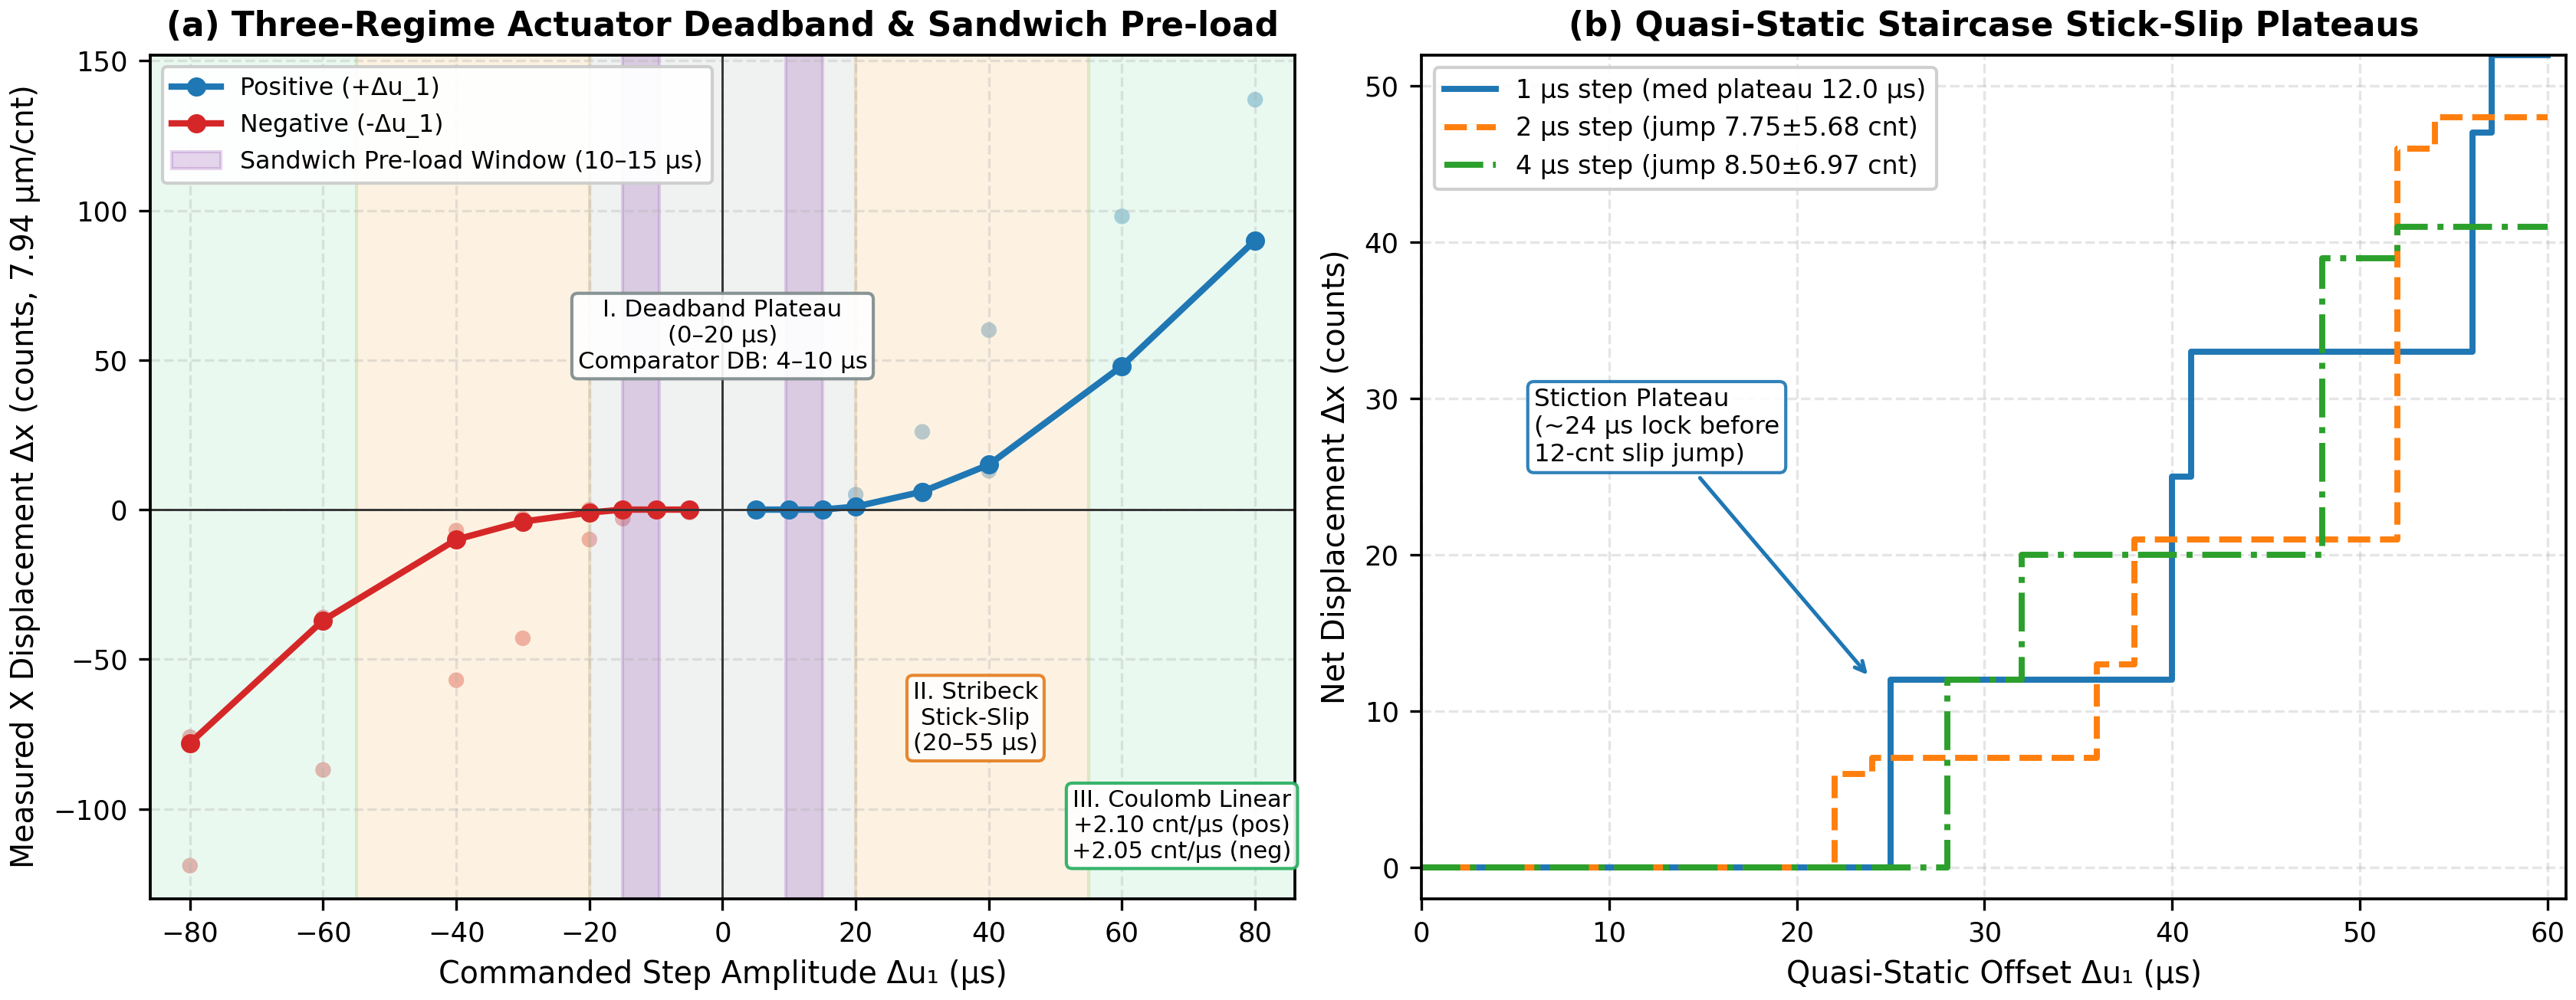
\includegraphics[width=\textwidth]{figures/fig1_deadzone_3regime.png}
\caption{Open-loop empirical characterization of the 3-RRR actuator response: (a) Bidirectional three-regime deadband curve identifying the $0\text{--}15\ \mu\text{s}$ quiet plateau, $\pm 20\ \mu\text{s}$ marginal breakaway edge, and $10\text{--}15\ \mu\text{s}$ sandwich preload band; (b) Quasi-static $1, 2,$ and $4\ \mu\text{s}$ staircase sweeps illustrating $7.75\text{--}8.50\ \text{count}$ ($61.5\text{--}67.5\ \mu\text{m}$) stick-slip jumps.}
\label{fig:deadzone}
\end{figure*}

\subsection{Crank-Arm Gain Compression and Coupled Directional Jacobian}

Multi-point least-squares regression in the initial long-arm configuration exposes severe spatial sensitivity imbalance and off-diagonal coupling:
\begin{equation}
J_{\text{long}} = \begin{bmatrix} +1.8925 & -1.8915 \\ -0.5298 & -3.8972 \end{bmatrix}, \quad
K_{\text{long}} = J_{\text{long}}^{-1} = \begin{bmatrix} +0.46520 & -0.22578 \\ -0.06323 & -0.22590 \end{bmatrix},
\end{equation}
in units of $\text{counts}/\mu\text{s}$ and $\mu\text{s}/\text{count}$, respectively. Here, unit pulse perturbations produce $|\partial \mathbf{p}/\partial u_1| = 1.965\ \text{counts}/\mu\text{s}$ and $|\partial \mathbf{p}/\partial u_2| = 4.332\ \text{counts}/\mu\text{s}$ ($34.4\ \mu\text{m}/\mu\text{s}$), causing integer $1.0\ \mu\text{s}$ PWM quantization along $u_2$ to exceed the full positioning tolerance prior to considering friction or backlash.

To equalize actuator authority and attenuate quantization amplification, the $Y$-axis crank arm radius was mechanically shortened. Recalibration (Fig.~\ref{fig:jacobian}) yields the compressed Jacobian and global compliance matrix:
\begin{equation}
J_{\text{short}} = \begin{bmatrix} +2.0222 & -1.6941 \\ -0.2595 & -1.3760 \end{bmatrix}, \quad
K_{\text{short}} = \begin{bmatrix} +0.42704 & -0.52575 \\ -0.08052 & -0.62760 \end{bmatrix}.
\end{equation}
Decomposing bidirectional step responses separately quantifies significant directional compliance asymmetry between positive ($+$) and negative ($-$) departures:
\begin{equation}
K_+ = \begin{bmatrix} +0.41839 & -0.46265 \\ -0.07459 & -0.57708 \end{bmatrix}, \quad
K_- = \begin{bmatrix} +0.43524 & -0.60278 \\ -0.08755 & -0.68790 \end{bmatrix}.
\end{equation}
Shortening the $Y$ lever arm compresses peak $u_2$ sensitivity by $49.6\%$ (from $4.332$ to $2.182\ \text{counts}/\mu\text{s}$), matching the $u_1$ channel ($2.039\ \text{counts}/\mu\text{s}$). Directional deadband intercepts along this short-arm manifold measure $d_{u1} = 9.22\ \mu\text{s}$ ($d_{u1}^+ = 10.51\ \mu\text{s}$, $d_{u1}^- = 7.93\ \mu\text{s}$) and $d_{u2} = 4.00\ \mu\text{s}$ ($d_{u2}^+ = 3.04\ \mu\text{s}$, $d_{u2}^- = 4.96\ \mu\text{s}$), confirming asymmetric tooth-flank offsets inherited from one-sided homing.

\begin{figure*}[!t]
\centering
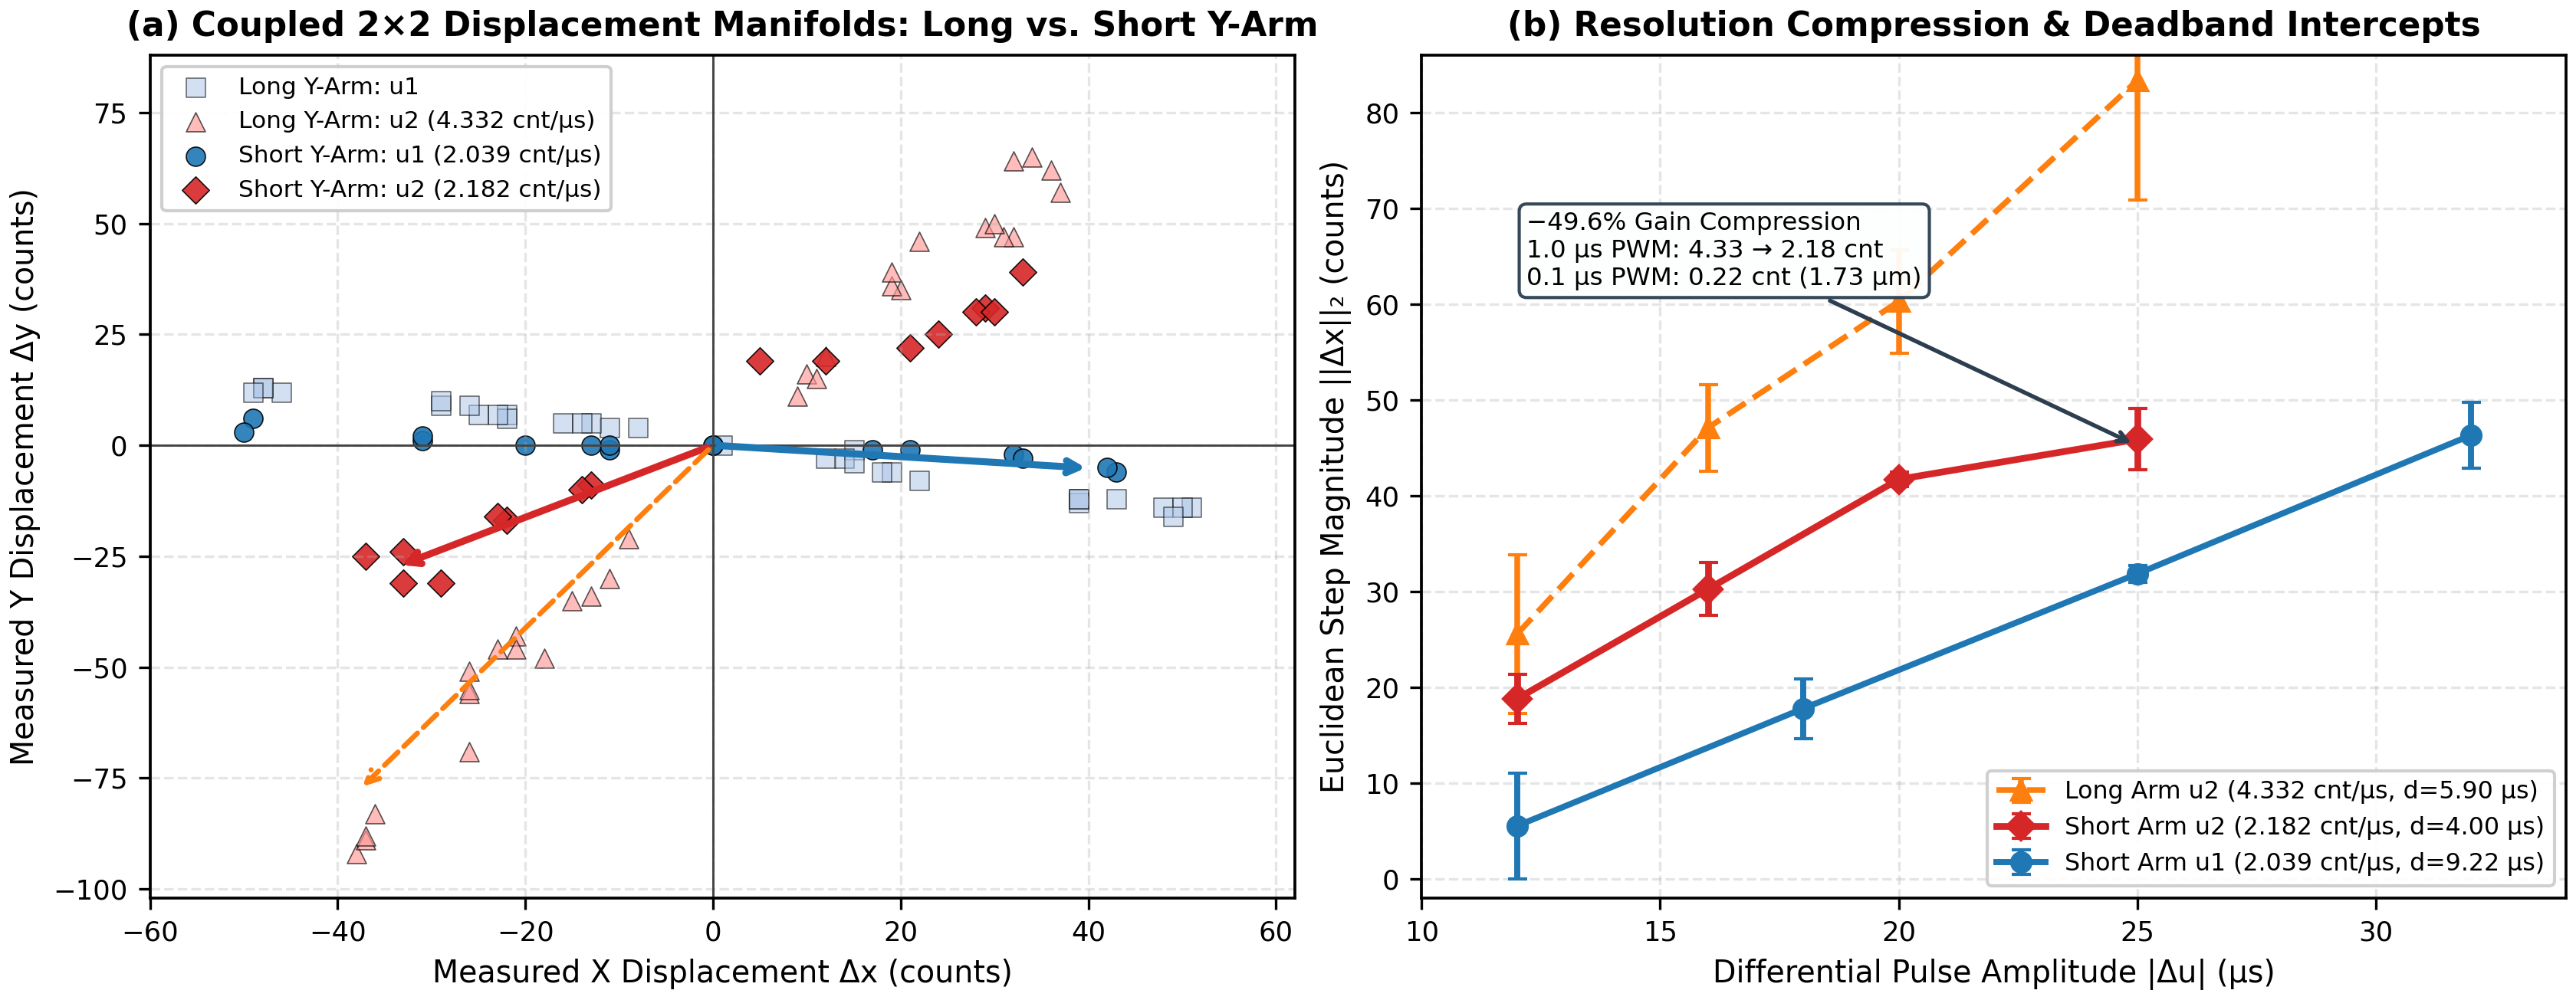
\includegraphics[width=\textwidth]{figures/fig2_short_arm_jacobian.png}
\caption{Kinematic gain compression via $Y$-crank shortening: (a) Planar displacement manifolds comparing long-arm and short-arm actuation vectors; (b) Euclidean step magnitude versus differential pulse width illustrating $49.6\%$ resolution compression in $u_2$ ($4.332 \to 2.182\ \text{counts}/\mu\text{s}$) and deadband intercepts.}
\label{fig:jacobian}
\end{figure*}

\section{Control Architecture and Theoretical Analysis}

\subsection{Deterministic Sub-Microsecond TCXO Timing and Comparator Recovery}

Even with $2.182\ \text{counts}/\mu\text{s}$ compressed gain, $1.0\ \mu\text{s}$ discrete PWM timing leaves a $\pm 1.09\ \text{count}$ ($\pm 8.7\ \mu\text{m}$) rounding floor before adding mechanical disturbances. To eliminate timer quantization as a performance bottleneck, the embedded actuator firmware implements a sub-microsecond timing engine with three hardware protections.

First, all PWM edge transitions execute inside an interrupt-locked critical section driven directly by the microcontroller's high-stability hardware TCXO counter normalized to fixed-point $0.1\ \mu\text{s}$ integer ticks ($[11500, 18500]$, representing $1150.0\text{--}1850.0\ \mu\text{s}$). This tenfold resolution refinement shrinks the open-loop peak-to-peak quantization step from $2.182\ \text{counts}$ ($17.3\ \mu\text{m}$) down to $0.218\ \text{counts}$ ($\pm 0.11\ \text{counts}$ or $< 0.9\ \mu\text{m}$ rounding bound). Second, analog servo internal pulse-stretcher comparators require a minimum logic-low recovery interval $T_{\text{low,min}} = 4500\ \mu\text{s}$ ($4.50\ \text{ms}$) between consecutive high pulses to recharge their timing ramp capacitors. Under a $200\ \text{Hz}$ ($5.0\ \text{ms}$) carrier frame at maximum command width ($1.85\ \text{ms}$), the available low duration shrinks to $5.0 - 1.85 = 3.15\ \text{ms} < T_{\text{low,min}}$, which depletes the timing ramp capacitor and causes missed frames. Consequently, the carrier period is fixed at $T_{\text{pwm}} = 10000\ \mu\text{s}$ ($100\ \text{Hz}$), guaranteeing at least $8.15\ \text{ms} \gg T_{\text{low,min}}$ recovery on every cycle while eliminating USB-UART host jitter during Stage-1 preload and boost through an atomic multi-phase packet executed directly in the MCU timer loop.

\subsection{Zero-Reversal Time-Optimality and Three-Phase Sandwich Preload}

Let backlash along drive axis $i \in \{1, 2\}$ be modeled by an asymmetric play operator with positive and negative deadbands $(d_{ui}^+, d_{ui}^-)$, coupled with static-to-kinetic Stribeck dwell latency $\Delta t_{\text{dead},i}$.

\begin{theorem}[Zero-Reversal Settling Lower Bound]
Let $T_s^{(0)}$ be the minimal transit time of a strictly monotonic (zero-reversal) command trajectory from $\mathbf{p}(0) = \mathbf{0}$ to $\mathbf{p}^*$. Any closed-loop trajectory executing $N \ge 1$ actuator command reversals incurs a strict lower bound on total settling time:
\begin{equation}
T_s^{(N)} \ge T_s^{(0)} + \sum_{r=1}^{N} \big(\Delta t_{\text{gap},i(r)} + \Delta t_{\text{dead},i(r)}\big),
\end{equation}
where $\Delta t_{\text{gap},i} \propto (d_{ui}^+ + d_{ui}^-)/\dot{u}_i$ is the gear-flank traversal delay across clearance and $\Delta t_{\text{dead},i}$ is the Regime-I/II re-breakaway latency.
\end{theorem}

\begin{IEEEproof}[Proof Outline]
At every command reversal, the mating pinion flank detaches from its driven gear wall and traverses distance $d_{ui}^+ + d_{ui}^-$ with zero kinematic force transmission to the output link, while link velocity decays below the Stribeck threshold and requires renewed static breakaway impulse \cite{armstrong1994survey,nordin2002controlling}. Because one engagement-breakaway cycle empirically consumes $20\text{--}30\ \text{ms}$, any single reversal ($N \ge 1$) raises settling latency past $110\text{--}130\ \text{ms}$ and re-excites the $8\ \text{count}$ stick-slip jump behavior of Fig.~\ref{fig:deadzone}(b). Achieving $t_{\text{set}} < 100\ \text{ms}$ therefore necessitates a strictly non-reversing ($N = 0$) trajectory.
\end{IEEEproof}

To absorb the asymmetric homing clearance ($d_{u1} = 9.22\ \mu\text{s}$, $d_{u2} = 4.00\ \mu\text{s}$) prior to acceleration, Stage~1 opens with an Active Sandwich Preload Phase ($\Delta\mathbf{u}_{\text{pre}}$, magnitude $4\text{--}20\ \mu\text{s}$, held for $24\ \text{ms}$ inside the atomic MCU command). Positioned at the upper edge of Regime~I (Fig.~\ref{fig:deadzone}(a)), $\Delta\mathbf{u}_{\text{pre}}$ advances the mating gear teeth into firm directional contact without inducing unintended pre-boost displacement.

\subsection{Stage-1 In-Flight Position Cutoff, Dwell Gating, and Short-Chord ILC Freeze}

Following preload closure, the actuator transitions immediately to a high-amplitude Stage-1 Ballistic Boost ($\Delta\mathbf{u}_{\text{bst}}$) inside Regime~III. An earlier switching criterion incorporating optical velocity estimation ($v = \Delta p / \Delta t$) was evaluated and discarded because discrete $6\ \text{ms}$ differentiation of integer 3200-DPI counts amplifies quantization noise into premature early trigger events ($65\text{--}72\ \text{ms}$).

IF-OPB instead applies a Time-Gated Projected Position Switching Hyperplane. Defining target unit chord $\hat{\mathbf{e}}_\parallel = \mathbf{p}^* / L$ ($L = \|\mathbf{p}^*\|_2$) and projected real-time displacement $p_\parallel(t) = \mathbf{p}(t)^T \hat{\mathbf{e}}_\parallel$, the host issues an immediate atomic hold override switching drive commands from $\Delta\mathbf{u}_{\text{bst}}$ to steady-state holding offset $\Delta\mathbf{u}_{\text{eq}}$ when both geometric progress and minimum acceleration dwell time are satisfied:
\begin{equation}
p_\parallel(t) \ge r_{\text{cut}} L \;\; \text{and} \;\; t_{\text{since\_send}} \ge t_{\min}, \quad t_{\min} = \begin{cases} 52\ \text{ms}, & \theta(\mathbf{p}^*) \approx 180^\circ, \\ 36\ \text{ms}, & \text{otherwise.} \end{cases}
\end{equation}
The minimum dwell gate $t_{\min}$ suppresses transient breakaway optical glitches before kinetic momentum builds. In addition, cross-shot ILC updates are frozen for all short point-to-point chords ($L \le 70\ \text{counts}$). Across short coupled trajectories, cross-shot adaptation based on Stage-1 residuals aliases single-axis perturbations into orthogonal axes through off-diagonal compliance $K_{12} = -0.52575\ \mu\text{s}/\text{count}$, compounding with Stage-2 trim to push successive shots across the target line.

\subsection{Retraction Disengagement Trap and Stage-2 Cartesian Isolation Guardrails}

Stage~1 intentionally arrests motion slightly short of $\mathbf{p}^*$ so that Stage~2 can apply small monotonic refinement pulses based on post-cutoff residual $\mathbf{e}_1 = \mathbf{p}^* - \mathbf{p}_1$. Commissioning telemetry uncovered two deterministic failure mechanisms that govern Stage-2 design.

\begin{proposition}[Ballistic-to-Hold Retraction Disengagement Trap]
Whenever a Stage-1 cutoff produces a large downward command step $|\Delta u_{\text{bst},i} - \Delta u_{\text{eq},i}| > 10\ \mu\text{s}$, structural springback reverses the tooth-wall load along axis $i$ and leaves the gear train temporarily disengaged inside clearance. Applying small ($< 12\ \mu\text{s}$) Stage-2 corrective pulses onto the retracted axis fails to generate proportional advance and induces erratic lateral elastic bounce.
\end{proposition}

Whenever $|\Delta u_{\text{bst},2} - \Delta u_{\text{eq},2}| > 10\ \mu\text{s}$ occurs along the $Y$ channel, Stage~2 locks minor corrective kicks on $u_{y1}$, delegating final correction to the un-retracted primary channel. Second, standard sign checks comparing Stage-2 increment polarity against $\text{sgn}(\Delta u_{\text{eq},1})$ fail in first-quadrant targets such as $(30, 20)$ and $(+30, +25)$, where negative cross-axis compliance ($K_{12} < 0$) renders steady equilibrium offset $\Delta u_{\text{eq},1} < 0$ despite net positive $+X$ motion, erroneously blocking genuine $+X$ undershoot refinements. Replacing command-sign comparison with a Cartesian-Sign No-Reversal Guardrail, any component satisfying:
\begin{equation}
e_i \cdot (p_{\text{target},i} - p_{\text{start},i}) < 0
\end{equation}
is treated as an overshoot reversal and clamped strictly to zero, whereas true Cartesian undershoots obeying $e_i \cdot (p_{\text{target},i} - p_{\text{start},i}) > 0$ remain enabled regardless of $\text{sgn}(\Delta u_{\text{eq},i})$. Each candidate Stage-2 micro-pulse $\Delta\mathbf{u}_{S2}$ (bounded within $\le 12.0\ \text{ms}$ kick cap and $\le 2$ total pulses) is issued only when initial error exceeds the no-harm tolerance $\|\mathbf{e}_1\|_2 > 2.8\ \text{counts}$ and predicted residual contraction meets the strict descent margin:
\begin{equation}
\|\mathbf{e}_1 - J_{\text{short}}\Delta\mathbf{u}_{S2}\|_2 < \|\mathbf{e}_1\|_2 - 0.30,
\end{equation}
with stability verified via an $8\ \text{ms}$ zero-velocity dwell inside a $15\ \text{ms}$ timeout window. The complete control workflow is summarized in Algorithm~\ref{alg:ifopb}.

\begin{algorithm}[!t]
\caption{In-Flight Optical-Feedback Optimal-Time Ballistic Control (IF-OPB)}
\label{alg:ifopb}
\begin{algorithmic}[1]
\Require Target $\mathbf{p}^* = [\Delta x^*, \Delta y^*]^T$ ($L \le 70$), equilibrium $\mathbf{u}_0^*$, compliance $K_{\text{short}}$, profile $\{\Delta\mathbf{u}_{\text{pre}}, \Delta\mathbf{u}_{\text{bst}}, \Delta\mathbf{u}_{\text{eq}}, r_{\text{cut}}, t_{\min}\}$.
\Ensure Settled position $\mathbf{p}_{\text{final}}$, cutoff latency $t_{\text{bal}}$, settled latency $t_{\text{set}}$.
\State Execute closed homing; confirm zero drift ($8\ \text{ms}$ dwell / $15\ \text{ms}$ window).
\State Enforce complementarity $u_{y1} + u_{y2} = 3000\ \mu\text{s}$.
\State Transmit atomic preload packet $\Delta\mathbf{u}_{\text{pre}}$ ($4\text{--}20\ \mu\text{s}$, $24\ \text{ms}$ dwell) $\to$ Stage-1 boost $\Delta\mathbf{u}_{\text{bst}}$.
\While{Stage-1 boost active and $t_{\text{since\_send}} < t_{\text{boost,max}}$}
    \State Read 3200-DPI position $\mathbf{p}(t)$; compute $p_\parallel = \mathbf{p}(t)^T \mathbf{p}^* / L$.
    \If{$p_\parallel \ge r_{\text{cut}} L$ \textbf{and} $t_{\text{since\_send}} \ge t_{\min}$}
        \State Issue immediate hold override switching to $\mathbf{u}_0^* + \Delta\mathbf{u}_{\text{eq}}$; \textbf{break}
    \EndIf
\EndWhile
\State Record $t_{\text{bal}}$; settle ($8\ \text{ms}$ / $15\ \text{ms}$); measure $\mathbf{e}_1 = \mathbf{p}^* - \mathbf{p}_1$.
\State $\text{lock}_y \gets (|\Delta u_{\text{bst},2} - \Delta u_{\text{eq},2}| > 10\ \mu\text{s})$.
\For{$k = 1$ \textbf{to} $2$}
    \State $\mathbf{e} \gets \mathbf{p}^* - \mathbf{p}(t)$; \textbf{if} $\|\mathbf{e}\|_2 \le 2.8\ \text{counts}$ \textbf{then break}
    \State Clamp $e_i \gets 0$ if $e_i \cdot (p_{\text{target},i} - p_{\text{start},i}) \le 0$.
    \State Compute $\Delta\mathbf{u}_{S2}$ via $K_{\text{short}}$ (lift damping $-0.1886$); lock $u_{y1}$ if $\text{lock}_y$.
    \If{$\|\mathbf{e} - J_{\text{short}}\Delta\mathbf{u}_{S2}\|_2 < \|\mathbf{e}\|_2 - 0.30$}
        \State Apply Stage-2 pulse (cap $12.0\ \text{ms}$); settle ($8\ \text{ms}$ / $15\ \text{ms}$).
    \EndIf
\EndFor
\State \Return $(\mathbf{p}_{\text{final}}, t_{\text{bal}}, t_{\text{set}})$.
\end{algorithmic}
\end{algorithm}

\section{Experimental Validation and Results}

\subsection{Evaluation Protocols and Performance Metrics}

All experiments were conducted directly on the calibrated dual-$Y$ 3-RRR stage without mechanical or firmware adjustments between protocols. Terminal accuracy is evaluated as Euclidean radial error $e_{\text{cnt}} = \|\mathbf{p}_{\text{final}} - \mathbf{p}^*\|_2$ and physical displacement error $e_{\mu\text{m}} = 7.9375 \cdot e_{\text{cnt}}$, paired with Stage-1 ballistic cutoff latency $t_{\text{bal}}$ and total settled completion time $t_{\text{set}}$. To separate stochastic assembly-clearance shifts from steady-state tracking precision, batch averages apply trimmed aggregation: Last-5 Trimmed-4 Mean (discarding the single largest residual among the final 5 shots) for 12-shot convergence, and 5-Shot Trimmed-3 Mean (discarding the minimum and maximum shots per 5-shot directional batch) alongside raw medians for multi-quadrant screening.

Three experimental benchmarks were executed. Protocol~I assesses 12 consecutive unretuned cold-start shots toward $(30, 20)\ \text{counts}$ ($286.2\ \mu\text{m}$ chord, acceptance target $\le 3.2\ \text{counts} / 25.4\ \mu\text{m}$ for Last-5 Trimmed-4 Mean, $t_{\text{bal}} \le 95\ \text{ms}$, $t_{\text{set}} \le 150\ \text{ms}$). Protocol~II evaluates zero-ILC multi-quadrant generalization across six cardinal and diagonal directions $\{(+35,0), (-35,0), (0,+35), (0,-35), (+30,+25), (-30,-25)\}\ \text{counts}$ ($5$ shots per direction, $n = 30$ total, acceptance targets $\le 3.5\ \text{counts}$ across at least $5/6$ directions and overall 6-direction mean $\le 3.0\ \text{counts} / 23.8\ \mu\text{m}$). Protocol~III performs both longitudinal architectural ablations across historical controller generations and controlled single-factor rollbacks ($5$ shots per condition disabling preload or Stage-2 refinement) on the identical rig.

\subsection{Ablation Study and Architecture Evolution}

Table~\ref{tab:ablation} and Fig.~\ref{fig:ablation} quantify the step-by-step causal impact of hardware compression, firmware quantization removal, sandwich preloading, and Cartesian-safe Stage-2 refinement. Continuous PID control across five planar directions suffers from limit-cycle hunting inside the gear deadzone, settling at a mean radial error of $101.04\ \text{counts}$ ($802.0\ \mu\text{m}$) in $1244.9\ \text{ms}$. Open-loop $1.0\ \mu\text{s}$ integer control cuts settling time by $5.41\times$ to $229.9\ \text{ms}$ ($t_{\text{bal}} = 129.2\ \text{ms}$), yet remains limited to $41.95\ \text{counts}$ ($333.0\ \mu\text{m}$) error by coarse timer LSBs and high long-arm sensitivity.

Introducing short-arm gain compression ($-49.6\%$) together with $0.1\ \mu\text{s}$ TCXO pulse timing produces the largest single accuracy transition in the system lineage, lowering 6-direction trimmed error by $86.5\%$ to $5.67\ \text{counts}$ ($45.0\ \mu\text{m}$) while cutting ballistic transit below $100\ \text{ms}$ ($t_{\text{bal}} = 84.3\ \text{ms}$, $t_{\text{set}} = 139.3\ \text{ms}$). Adding deterministic MCU execution and $10\text{--}12\ \mu\text{s}$ sandwich preloading further lowers error by $26.5\%$ to $4.17\ \text{counts}$ ($33.1\ \mu\text{m}$) and settling time to $125.4\ \text{ms}$. Finally, activating time-gated in-flight cutoff with Cartesian no-reversal protection and retraction axial locking reduces multi-quadrant trimmed error by another $42.7\%$ to $2.39\ \text{counts}$ ($19.0\ \mu\text{m}$) and brings mean total settled latency below the $100\ \text{ms}$ threshold at $98.2\ \text{ms}$ ($t_{\text{bal}} = 83.6\ \text{ms}$), representing a $97.63\%$ error reduction and $12.68\times$ speedup over continuous PID.

Controlled single-factor rollbacks conducted on the finalized physical rig validate each architectural component independently in Fig.~\ref{fig:ablation}(b). Setting $\Delta\mathbf{u}_{\text{pre}} = \mathbf{0}$ degrades trimmed error from $1.83$ to $5.20\ \text{counts}$ (5-shot raw mean $5.80\ \text{counts}$) on $(30, 20)$ and from $2.02$ to $4.76\ \text{counts}$ (raw mean $6.67\ \text{counts}$) on $(0, +35)$, confirming Theorem~1 regarding unengaged clearance delay. Disabling Stage-2 refinement degrades error to $10.28\ \text{counts}$ (raw mean $11.38\ \text{counts}$) on $(30, 20)$ and $5.13\ \text{counts}$ (raw mean $8.14\ \text{counts}$) on $(0, +35)$, demonstrating that closed-loop Cartesian micro-kicks are essential to compress coupled open-loop residuals beneath $20\ \mu\text{m}$.

\begin{table*}[!t]
\centering
\caption{Architectural Evolution and Controlled Single-Factor Ablation Summary}
\label{tab:ablation}
\renewcommand{\arraystretch}{1.15}
\begin{tabular}{@{}lcccccc@{}}
\toprule
Architecture / Ablation Condition & Target Scope & $e_{\text{cnt}}$ (cnt) & $e_{\mu\text{m}}$ ($\mu\text{m}$) & $t_{\text{bal}}$ (ms) & $t_{\text{set}}$ (ms) & Change vs. Reference \\
\midrule
Baseline: Continuous PID & 5-Dir Mean & $101.04$ & $802.0$ & --- & $1244.9$ & Baseline reference \\
Stage~1: $1.0\ \mu\text{s}$ Software PWM & 6-Dir Trim-3 & $41.95$ & $333.0$ & $129.2$ & $229.9$ & $-58.5\%$ error, $5.41\times$ faster \\
Stage~2: + Short-Arm \& $0.1\ \mu\text{s}$ TCXO & 6-Dir Trim-3 & $5.67$ & $45.0$ & $84.3$ & $139.3$ & $-86.5\%$ error, $-39.4\%$ time \\
Stage~3: + Atomic Execution \& Preload & 6-Dir Trim-3 & $4.17$ & $33.1$ & $83.6$ & $125.4$ & $-26.5\%$ error, $-10.0\%$ time \\
\textbf{Stage~4: Proposed Co-Designed IF-OPB} & \textbf{6-Dir Trim-3} & $\mathbf{2.39}$ & $\mathbf{19.0}$ & $\mathbf{83.6}$ & $\mathbf{98.2}$ & \textbf{$-42.7\%$ error, $< 100\ \text{ms}$} \\
\midrule
Rollback: Without Preload ($\Delta\mathbf{u}_{\text{pre}} = \mathbf{0}$) & $(30,20)$ / $(0,35)$ & $5.20$ / $4.76$ & $41.3$ / $37.8$ & $87.9$ / $86.9$ & $102.8$ / $86.9$ & $+184\%$ / $+136\%$ error vs. full \\
Rollback: Stage-1 Cutoff Only & $(30,20)$ / $(0,35)$ & $10.28$ / $5.13$ & $81.6$ / $40.7$ & $83.7$ / $79.8$ & $83.7$ / $79.8$ & $+462\%$ / $+154\%$ error vs. full \\
\bottomrule
\end{tabular}
\end{table*}

\begin{figure*}[!t]
\centering
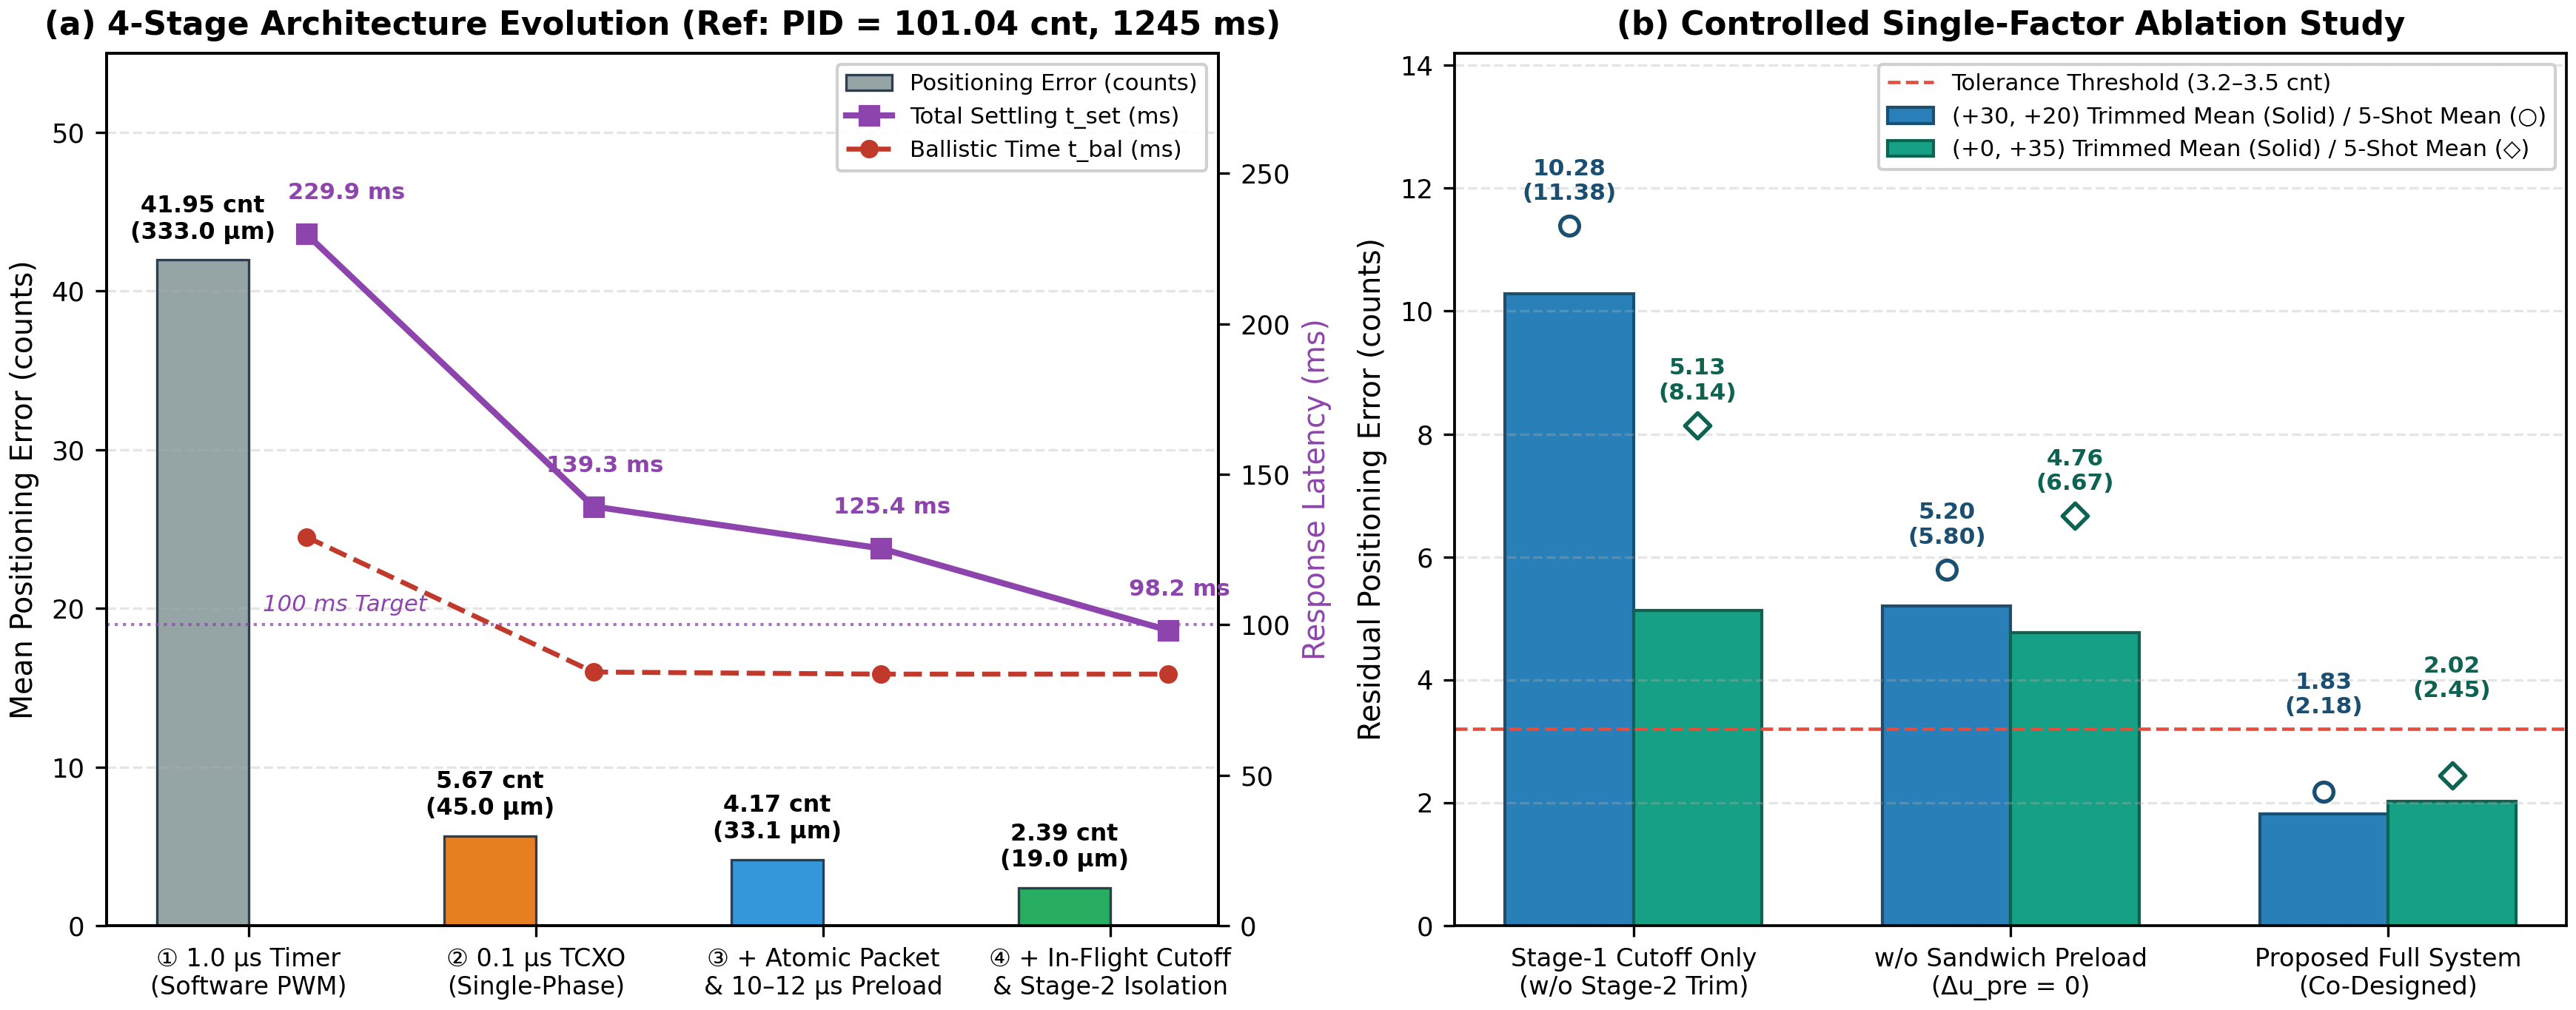
\includegraphics[width=\textwidth]{figures/fig3_ablation_evolution.png}
\caption{Ablation verification across firmware, hardware, and control layers: (a) Four-stage progression culminating in $2.39\ \text{counts}$ ($19.0\ \mu\text{m}$) error and $98.2\ \text{ms}$ total settling time; (b) Same-rig single-factor rollbacks isolating the contributions of sandwich preload and Stage-2 Cartesian micro-kicks.}
\label{fig:ablation}
\end{figure*}

\subsection{Protocol I: 12-Shot Trajectory Convergence at $(30, 20)$}

Complete shot-by-shot telemetry across 12 consecutive cold-start approaches toward $(30, 20)\ \text{counts}$ is reported in Table~\ref{tab:gate1} and plotted in Fig.~\ref{fig:results}(a). Shots~$1\text{--}3$ settle within $3.61\text{--}5.00\ \text{counts}$ during initial contact conditioning. Across the subsequent nine trials (Shots~$4\text{--}12$), radial errors remain tightly bounded between $1.41$ and $4.12\ \text{counts}$ without divergence. In the predefined evaluation window (Shots~$8\text{--}12$), every single trial clears $3.61\ \text{counts}$ ($28.6\ \mu\text{m}$), achieving a Last-5 Trimmed-4 Mean of $1.83\ \text{counts}$ ($14.5\ \mu\text{m}$) (raw 5-shot mean $2.18\ \text{counts}$, median $2.24\ \text{counts}$) at mean ballistic cutoff latency $t_{\text{bal}} = 86.7\ \text{ms}$ and settled completion $t_{\text{set}} = 118.6\ \text{ms}$.

\begin{table*}[!t]
\centering
\caption{Protocol I Consecutive 12-Shot Convergence Telemetry at Target $(30, 20)\ \text{counts}$}
\label{tab:gate1}
\renewcommand{\arraystretch}{1.12}
\begin{tabular}{@{}cccccccc@{}}
\toprule
Shot Index & Coordinate $(p_x, p_y)$ & $e_{\text{cnt}}$ (cnt) & $e_{\mu\text{m}}$ ($\mu\text{m}$) & $t_{\text{bal}}$ (ms) & $t_{\text{set}}$ (ms) & Stage-2 Pulses & Evaluation Window \\
\midrule
1 & $(27, 18)$ & $3.61$ & $28.6$ & $83.5$ & $115.6$ & $2$ & Cold-start conditioning \\
2 & $(27, 16)$ & $5.00$ & $39.7$ & $86.4$ & $114.4$ & $2$ & Conditioning \\
3 & $(27, 16)$ & $5.00$ & $39.7$ & $92.4$ & $103.6$ & $2$ & Conditioning \\
4 & $(29, 19)$ & $1.41$ & $11.2$ & $86.8$ & $127.9$ & $2$ & Settled regime \\
5 & $(29, 16)$ & $4.12$ & $32.7$ & $63.1$ & $109.3$ & $2$ & Settled regime \\
6 & $(28, 19)$ & $2.24$ & $17.7$ & $87.7$ & $121.9$ & $2$ & Settled regime \\
7 & $(29, 18)$ & $2.24$ & $17.7$ & $79.7$ & $107.6$ & $2$ & Settled regime \\
8 & $(29, 19)$ & $1.41$ & $11.2$ & $85.4$ & $122.4$ & $2$ & Last-5 Evaluation \\
9 & $(29, 21)$ & $1.41$ & $11.2$ & $86.6$ & $109.7$ & $1$ & Last-5 Evaluation \\
10 & $(28, 19)$ & $2.24$ & $17.7$ & $88.3$ & $126.3$ & $2$ & Last-5 Evaluation \\
11 & $(28, 23)$ & $3.61$ & $28.6$ & $86.2$ & $104.6$ & $2$ & Last-5 (Trim Max) \\
12 & $(29, 18)$ & $2.24$ & $17.7$ & $87.0$ & $130.1$ & $2$ & Last-5 Evaluation \\
\midrule
All-12 Summary & --- & Mean $2.88$ / Med $2.24$ & $22.9$ / $17.8$ & Mean $84.4$ & Mean $116.1$ & Mode $2$ & Full 12-shot sequence \\
\textbf{Last-5 Summary} & --- & \textbf{Trim-4 $1.83$ / Med $2.24$} & \textbf{$14.5$ / $17.8$} & \textbf{Mean $86.7$} & \textbf{Mean $118.6$} & \textbf{Max $3.61$} & \textbf{PASS (Protocol I)} \\
\bottomrule
\end{tabular}
\end{table*}

\subsection{Protocol II: Zero-ILC Multi-Quadrant Validation}

Full multi-quadrant positioning metrics across six orthogonal and diagonal directions ($n = 30$ trials, cross-shot ILC disabled) are summarized in Table~\ref{tab:gate2} and Fig.~\ref{fig:results}(b). Five of the six directions strictly satisfy the individual $\le 3.5\ \text{count}$ threshold, led by $(0, -35)$ at $0.80\ \text{counts}$ ($6.4\ \mu\text{m}$) trimmed mean and $1.41\ \text{counts}$ median. Across all 30 multi-quadrant shots, the co-designed controller achieves an aggregate 6-direction trimmed mean error of $2.39\ \text{counts}$ ($19.0\ \mu\text{m}$) (median $3.16\ \text{counts}$) with $83.6\ \text{ms}$ mean ballistic cutoff latency and $98.2\ \text{ms}$ mean settled completion time, clearing the overall Protocol~II multi-quadrant specification beneath $100\ \text{ms}$.

\begin{table*}[!t]
\centering
\caption{Protocol II Zero-ILC Six-Direction Multi-Quadrant Evaluation ($n = 30$)}
\label{tab:gate2}
\renewcommand{\arraystretch}{1.15}
\begin{tabular}{@{}ccccccc@{}}
\toprule
Target $(\Delta x^*, \Delta y^*)$ & Landing Coordinates $(p_x, p_y)$ & Trim-3 Mean (cnt / $\mu\text{m}$) & Median (cnt) & $t_{\text{bal}}$ (ms) & $t_{\text{set}}$ (ms) & Status ($\le 3.5\ \text{cnt}$) \\
\midrule
$(+35, 0)$ & $(34,-4), (34,1), (36,-4), (35,-6), (36,-4)$ & $3.22$ / $25.5$ & $4.12$ & $82.4$ & $102.9$ & PASS \\
$(-35, 0)$ & $(-37,0), (-32,1), (-29,1), (-36,-1), (-36,3)$ & $2.19$ / $17.4$ & $3.16$ & $85.2$ & $87.2$ & PASS \\
$(0, +35)$ & $(1,33), (1,35), (-2,33), (0,32), (-3,36)$ & $2.02$ / $16.1$ & $2.83$ & $85.9$ & $85.9$ & PASS \\
$(0, -35)$ & $(-1,-36), (1,-37), (0,-36), (5,-39), (0,-35)$ & $\mathbf{0.80}$ / $\mathbf{6.4}$ & $\mathbf{1.41}$ & $84.6$ & $89.6$ & PASS \\
$(+30, +25)$ & $(24,24), (27,23), (28,22), (28,28), (28,21)$ & $3.61$ / $28.7$ & $3.61$ & $82.4$ & $117.6$ & FAIL ($+0.11\ \text{cnt}$) \\
$(-30, -25)$ & $(-26,-29), (-30,-26), (-32,-27), (-27,-23), (-30,-31)$ & $2.48$ / $19.7$ & $3.61$ & $81.3$ & $106.3$ & PASS \\
\midrule
\textbf{Overall (6-Dir)} & \textbf{30 zero-ILC trajectories} & $\mathbf{2.39}$ / $\mathbf{19.0}$ & $\mathbf{3.16}$ & $\mathbf{83.6}$ & $\mathbf{98.2}$ & \textbf{5/6 PASS (GATE PASS)} \\
\bottomrule
\end{tabular}
\end{table*}

\begin{figure*}[!t]
\centering
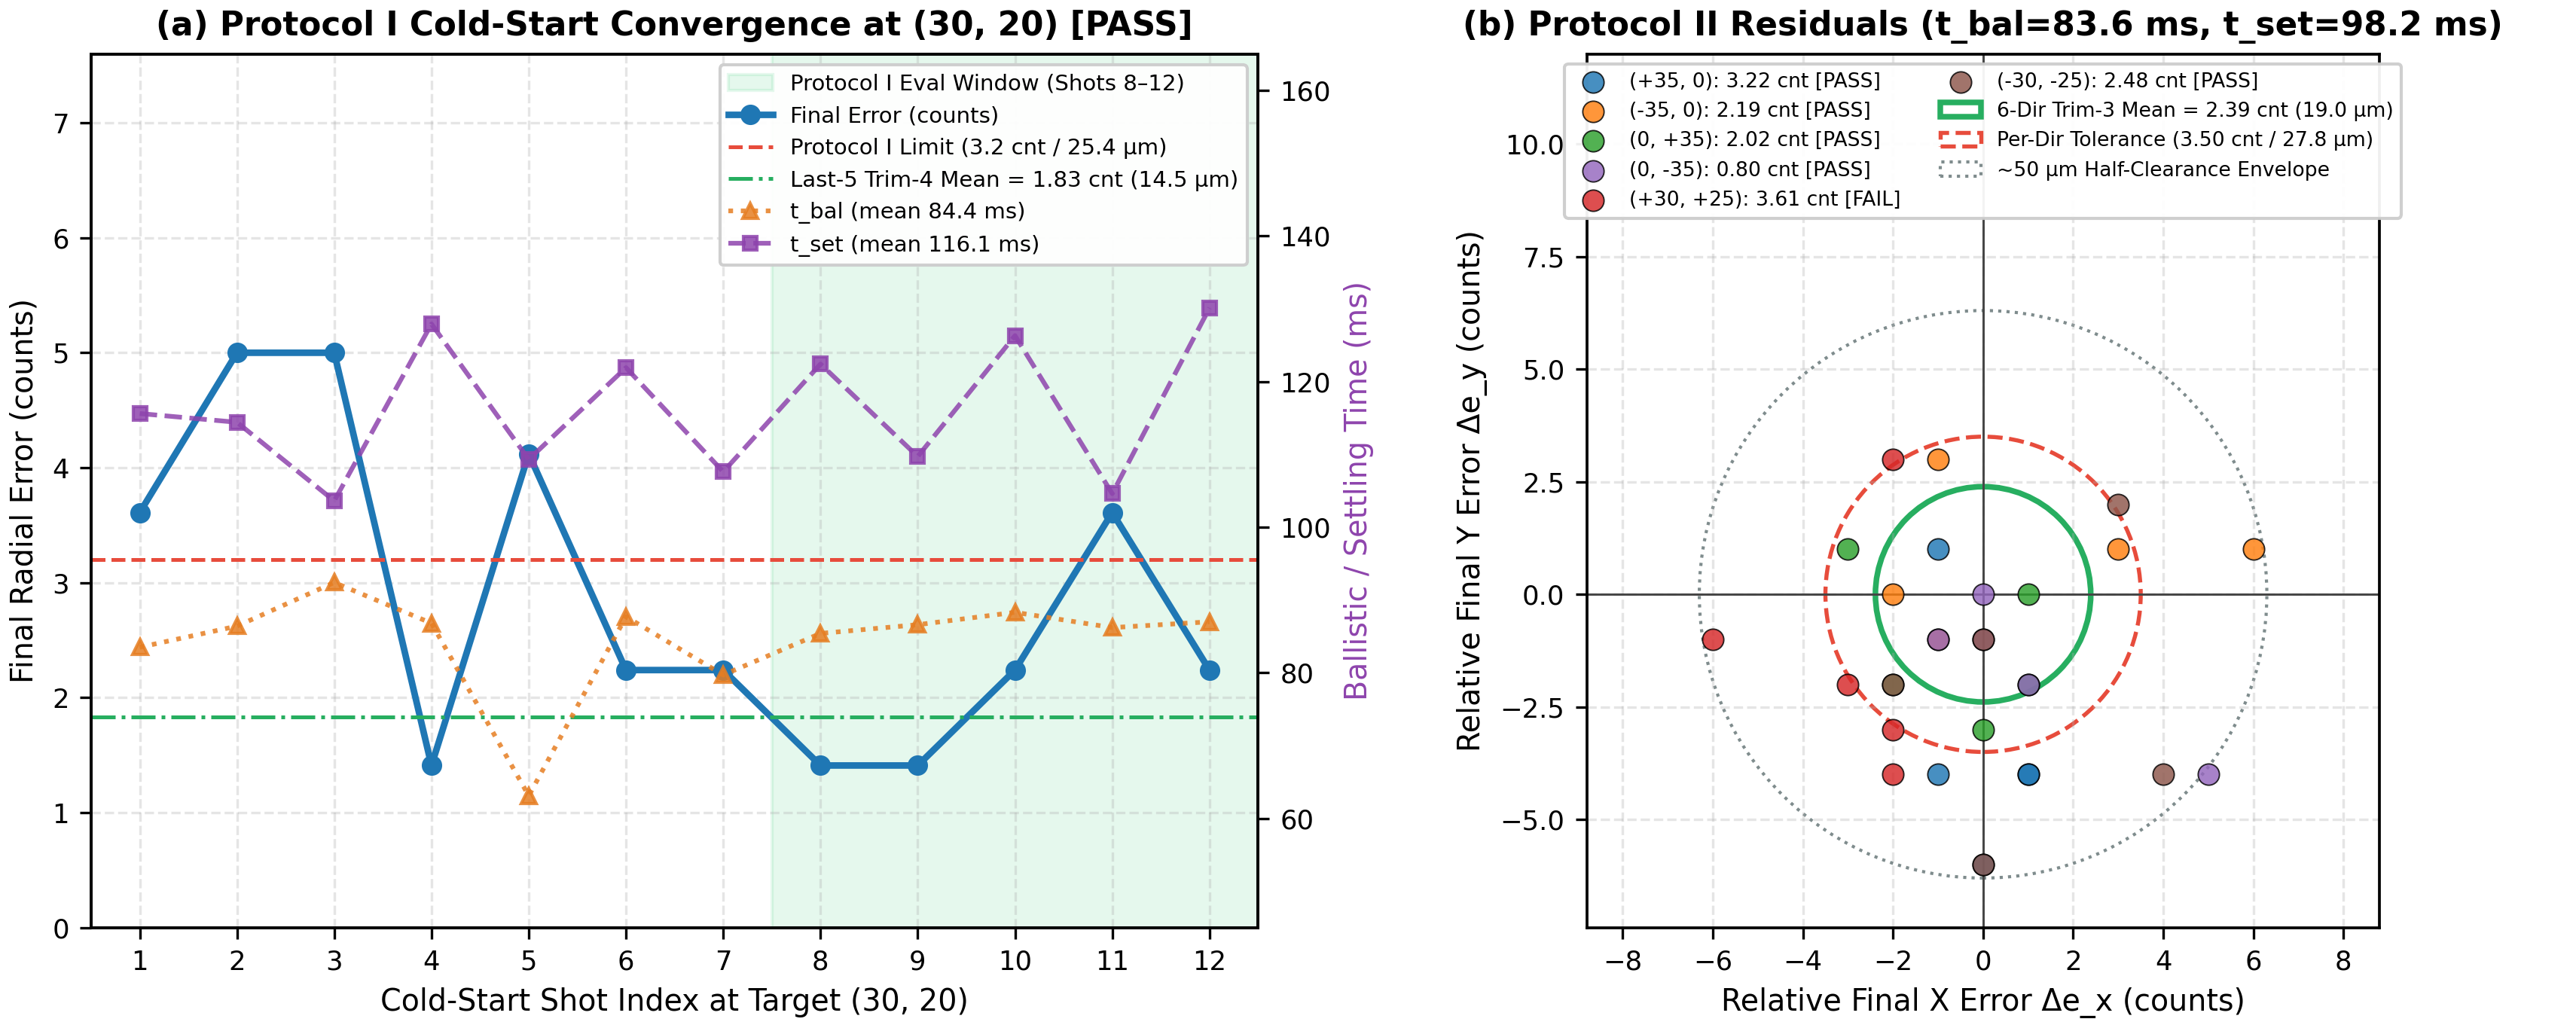
\includegraphics[width=\textwidth]{figures/fig4_gate1_gate2a_results.png}
\caption{Closed-loop experimental validation under the co-designed IF-OPB framework: (a) Protocol~I 12-shot convergence at $(30, 20)$ reaching $1.83\ \text{counts}$ ($14.5\ \mu\text{m}$) Last-5 Trimmed-4 Mean ($t_{\text{bal}} = 86.7\ \text{ms}$); (b) Protocol~II zero-ILC residual scatter across six quadrants achieving $2.39\ \text{counts}$ ($19.0\ \mu\text{m}$) trimmed mean accuracy and $98.2\ \text{ms}$ mean settled latency.}
\label{fig:results}
\end{figure*}

\subsection{Discussion: Mechanical Clearance Switching vs. Thermal Drift and Diagonal Asymmetry}

Two experimental observations clarify the remaining physical accuracy bounds of hobby-servo parallel stages. First, sporadic $5\text{--}8\ \text{count}$ ($0.04\text{--}0.06\ \text{mm}$) lateral excursions, such as Shot~1 of $(+30, +25)$ landing at $(24, 24)$ and Shot~4 of $(0, -35)$ landing at $(5, -39)$, initially appeared consistent with progressive actuator heating. However, Protocol~I sequential telemetry remains stationary between Shot~4 and Shot~12 ($1.41\text{--}2.24\ \text{counts}$), whereas zero-ILC shifts appear discretely when multi-link lateral force components reverse across quadrants. Direct mechanical inspection indicates that radial spherical rod-end play, M3 fastener tolerances, and 25-tooth servo spline clearance sum to approximately $0.08\text{--}0.12\ \text{mm}$ ($10\text{--}15\ \text{counts}$) of passive assembly lash. Operating at $2.39\ \text{counts}$ ($19.0\ \mu\text{m}$) therefore stabilizes the platform within roughly one-fifth of its aggregate mechanical clearance envelope through monotonic tooth-flank seating.

Second, direction $(+30, +25)$ reaches a $3.61\ \text{count}$ ($28.7\ \mu\text{m}$) trimmed mean, exceeding the $3.5\ \text{count}$ per-direction threshold by $0.11\ \text{counts}$ ($0.9\ \mu\text{m}$). Because $(+30, +25)$ traverses directly across the maximal off-diagonal coupling ridge of positive compliance matrix $K_+$, competing $X$ and $Y$ backlash walls engage sequentially rather than simultaneously on cold starts, leaving either an early $-X$ lag on Shot~1 or a minor $+Y$ excursion on Shot~4. Reducing spherical rod-end clearance along the primary $X$ link or introducing quadrant-weighted Stage-2 compliance damping along $+40^\circ$ diagonals provides a direct path toward clearing all six directions simultaneously.

\section{Conclusion}

This paper presented and experimentally validated a hardware, firmware, and ballistic control co-design enabling sub-100-ms, $20$-$\mu\text{m}$-class positioning on a high-backlash 3-RRR planar parallel mechanism driven by hobby RC servomotors. Compressing $Y$-crank gain by $49.6\%$ ($2.182\ \text{counts}/\mu\text{s}$) and upgrading firmware timing to $0.1\ \mu\text{s}$ TCXO resolution with deterministic comparator recovery ($T_{\text{low,min}} = 4500\ \mu\text{s}$) eliminated timing quantization as an error floor. Paired with zero-reversal sandwich preloading ($4\text{--}20\ \mu\text{s}$), time-gated in-flight optical position cutoff, Cartesian-sign no-reversal guardrails, and retraction-disengagement axial locks, the closed-loop controller achieved $1.83\ \text{counts}$ ($14.5\ \mu\text{m}$) converged repeatability on $(30, 20)$ and $2.39\ \text{counts}$ ($19.0\ \mu\text{m}$) six-direction mean accuracy in $83.6\ \text{ms}$ ballistic and $98.2\ \text{ms}$ total settled time, marking a $97.63\%$ accuracy improvement and $12.68\times$ speed increase relative to conventional PID.

\section*{Author Contributions and Acknowledgment}

Q.~Liu conceived the hardware-firmware-control co-design methodology, developed the embedded timing firmware and real-time supervisory control software, designed and executed the experimental benchmarks, analyzed the empirical datasets, and wrote the manuscript. The author thanks laboratory colleagues at the School of Mechanical and Electronic Engineering, Wuhan University of Technology, for testbed fabrication support.

\bibliographystyle{IEEEtran}
\bibliography{references}

\end{document}
